
The different layers explained in the previous session are the divisions that can be made inside the code. But how is the system organized in term of processes and hardware? 
\paragraph{}
For instance for hardware there will be at least three different computers/types involved: 
\begin{itemize}
\item The computer of the therapist, used to display the progress of all patients and to communicate with them
\item Numerous computers of patients, used to work with the eCoach and to communicate with the therapist
\item Some kind of server used to facilitate the communication
\end{itemize}
You can also see this in figure ~\ref{fig:deploymentdiagram}.
\begin{figure}[H]
  \centering
  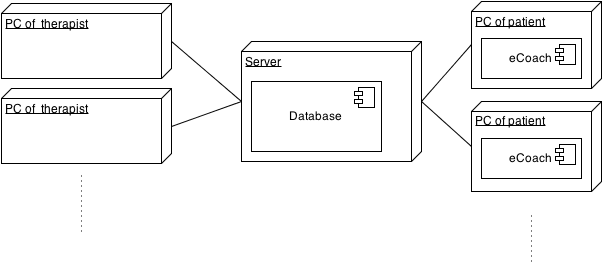
\includegraphics[width=\textwidth]{deployment-diagram.png}
  \caption{Deployment diagram of the system} 
  \label{fig:deploymentdiagram}
\end{figure}
On the computer of the therapist and on the computer of a patient a database system will run to store all the permanent user data (more about this in paragraph 2.3).  No decision has yet been made about what kind of database system is going to be used.

On the patient system a vizard process will run to display the avatars. Most of the view-layer (without the avatar displaying) and the control-layer is run from the same main process. 

Because the patient and the therapist do not share a computer and because the use of the program is very different for the patient and the therapist, separate programs are made for both users. This decreases the chance of security leaks and also decreases the amount of files to be installed locally.

